\documentclass[10pt]{article}

%%%%%%%%%%%%%%%%%%%%%%%%%%%%%%%%%%%%%%%%%%%%%%%%%%%%%%%%%%%%%%%%%%%%%%%%%%%%%%%%
% LaTeX Imports
%%%%%%%%%%%%%%%%%%%%%%%%%%%%%%%%%%%%%%%%%%%%%%%%%%%%%%%%%%%%%%%%%%%%%%%%%%%%%%%%
\usepackage{amsfonts}                                                   % Math fonts
\usepackage{amsmath}                                                    % Math formatting
\usepackage{amssymb}                                                    % Math formatting
\usepackage{amsthm}                                                     % Math Theorems
\usepackage{arydshln}                                                   % Dashed hlines
\usepackage{attachfile}                                                 % AttachFiles
\usepackage{cancel}                                                     % Cancelled math
\usepackage{caption}                                                    % Figure captioning
\usepackage{color}                                                      % Nice Colors
\input{./lib/dragon.inp}                                                % Tikz dragon curve
\usepackage[ampersand]{easylist}                                        % Easy lists
\usepackage{fancyhdr}                                                   % Fancy Header
\usepackage[T1]{fontenc}                                                % Specific font-encoding
%\usepackage[margin=1in, marginparwidth=2cm, marginparsep=2cm]{geometry} % Margins
\usepackage{graphicx}                                                   % Include images
\usepackage{hyperref}                                                   % Referencing
\usepackage[none]{hyphenat}                                             % Don't allow hyphenation
\usepackage{lipsum}                                                     % Lorem Ipsum Dummy Text
\usepackage{listings}                                                   % Code display
\usepackage{marginnote}                                                 % Notes in the margin
\usepackage{microtype}                                                  % Niceness
\usepackage{lib/minted}                                                 % Code display
\usepackage{multirow}                                                   % Multirow tables
\usepackage{pdfpages}                                                   % Include pdfs
\usepackage{pgfplots}                                                   % Create Pictures
\usepackage{rotating}                                                   % Figure rotation
\usepackage{setspace}                                                   % Allow double spacing
\usepackage{subcaption}                                                 % Figure captioning
\usepackage{tikz}                                                       % Create Pictures
\usepackage{tocloft}                                                    % List of Equations
%%%%%%%%%%%%%%%%%%%%%%%%%%%%%%%%%%%%%%%%%%%%%%%%%%%%%%%%%%%%%%%%%%%%%%%%%%%%%%%%
% Package Setup
%%%%%%%%%%%%%%%%%%%%%%%%%%%%%%%%%%%%%%%%%%%%%%%%%%%%%%%%%%%%%%%%%%%%%%%%%%%%%%%%
\hypersetup{%                                                           % Setup linking
    colorlinks=true,
    linkcolor=black,
    citecolor=black,
    filecolor=black,
    urlcolor=black,
}
\RequirePackage[l2tabu, orthodox]{nag}                                  % Nag about bad syntax
\renewcommand*\thesection{\arabic{section} }                             % Reset numbering
\renewcommand{\theFancyVerbLine}{ {\arabic{FancyVerbLine} } }              % Needed for code display
\renewcommand{\footrulewidth}{0.4pt}                                    % Footer hline
\setcounter{secnumdepth}{3}                                             % Include subsubsections in numbering
\setcounter{tocdepth}{3}                                                % Include subsubsections in toc
%%%%%%%%%%%%%%%%%%%%%%%%%%%%%%%%%%%%%%%%%%%%%%%%%%%%%%%%%%%%%%%%%%%%%%%%%%%%%%%%
% Custom commands
%%%%%%%%%%%%%%%%%%%%%%%%%%%%%%%%%%%%%%%%%%%%%%%%%%%%%%%%%%%%%%%%%%%%%%%%%%%%%%%%
\newcommand{\nvec}[1]{\left\langle #1 \right\rangle}                    %  Easy to use vector
\newcommand{\ma}[0]{\mathbf{A} }                                         %  Easy to use vector
\newcommand{\mb}[0]{\mathbf{B} }                                         %  Easy to use vector
\newcommand{\abs}[1]{\left\lvert #1 \right\rvert}                       %  Easy to use abs
\newcommand{\pren}[1]{\left( #1 \right)}                                %  Big parens
\let\oldvec\vec
\renewcommand{\vec}[1]{\oldvec{\mathbf{#1} } }                            %  Vector Styling
\newtheorem{thm}{Theorem}                                               %  Define the theorem name
\newtheorem{definition}{Definition}                                     %  Define the definition name
\definecolor{bg}{rgb}{0.95,0.95,0.95}
\newcommand{\java}[4]{\vspace{10pt}\inputminted[firstline=#2,
                                 lastline=#3,
                                 firstnumber=#2,
                                 gobble=#4,
                                 frame=single,
                                 label=#1,
                                 bgcolor=bg,
                                 linenos]{java}{#1} }
\newcommand{\python}[4]{\vspace{10pt}\inputminted[firstline=#2,
                                 lastline=#3,
                                 firstnumber=#2,
                                 gobble=#4,
                                 frame=single,
                                 label=#1,
                                 bgcolor=bg,
                                 linenos]{python}{#1} }
\newcommand{\js}[4]{\vspace{10pt}\inputminted[firstline=#2,
                                 lastline=#3,
                                 firstnumber=#2,
                                 gobble=#4,
                                 frame=single,
                                 label=#1,
                                 bgcolor=bg,
                                 linenos]{js}{#1} }
%%%%%%%%%%%%%%%%%%%%%%%%%%%%%%%%%%%%%%%%%%%%%%%%%%%%%%%%%%%%%%%%%%%%%%%%%%%%%%%%
% Beginning of document items - headers, title, toc, etc...
%%%%%%%%%%%%%%%%%%%%%%%%%%%%%%%%%%%%%%%%%%%%%%%%%%%%%%%%%%%%%%%%%%%%%%%%%%%%%%%%
\pagestyle{fancy}                                                       %  Establishes that the headers will be defined
\fancyhead[LE,LO]{Computer Systems Notes}                                  %  Adds header to left
\fancyhead[RE,RO]{Zoe Farmer}                                       %  Adds header to right
\cfoot{ \thepage }
\lfoot{CSCI 2400}
\rfoot{Han}
\title{Computer Systems Notes}
\author{Zoe Farmer}


\makeatletter
\global\let\tikz@ensure@dollar@catcode=\relax
\makeatother

%%%%%%%%%%%%%%%%%%%%%%%%%%%%%%%%%%%%%%%%%%%%%%%%%%%%%%%%%%%%%%%%%%%%%%%%%%%%%%%%
% Beginning of document items - headers, title, toc, etc...
%%%%%%%%%%%%%%%%%%%%%%%%%%%%%%%%%%%%%%%%%%%%%%%%%%%%%%%%%%%%%%%%%%%%%%%%%%%%%%%%
\pagestyle{fancy}                                                       %  Establishes that the headers will be defined
\fancyhead[LE,LO]{Lab Three}                                  %  Adds header to left
\fancyhead[RE,RO]{Zoe Farmer}                                       %  Adds header to right
\cfoot{\thepage}
\lfoot{APPM4560 - Markov Processes}
\rfoot{Manual Lladser}
\title{APPM 4560 Lab Three\\Simulating A Single Server Queue}
\author{Zoe Farmer}
\date{December 9, 2016}
%%%%%%%%%%%%%%%%%%%%%%%%%%%%%%%%%%%%%%%%%%%%%%%%%%%%%%%%%%%%%%%%%%%%%%%%%%%%%%%%
% Beginning of document items - headers, title, toc, etc...
%%%%%%%%%%%%%%%%%%%%%%%%%%%%%%%%%%%%%%%%%%%%%%%%%%%%%%%%%%%%%%%%%%%%%%%%%%%%%%%%
\begin{document}

\maketitle

The goal of this lab is to understand Markovian Queues.

Let $X = \pren{X_t}_{t \ge 0}$ denote the number of customers in an M/M/1-queue
with arrival rate $\lambda > 0$ and service rate $\mu > 0$. In addition, let $T
> 0$ be a fixed time.

\vspace{0.5cm}
\begin{easylist}[enumerate]
    @ What condition is necessary and sufficient for the queue to have a
    stationary distribution? What is it?
    \vspace{0.5cm}

    In  order for the queue to have a stationary distribution, $\lambda$ must be
    less than $\mu$. To put this in simpler terms, the rate of incoming events
    must be lower than the rate of outgoing, or else the system will infinitely
    increase. We can define a new parameter $\rho = \lambda / \mu$. This value
    must be less than $1$ in order for there to be a stationary distribution.

    Following the example in the book on page 160, we can find the stationary
    distribution to be the following.

    \begin{align*}
        \pi(n) =
        \pren{1 - \frac{\lambda}{\mu}}
        \pren{\frac{\lambda}{\mu}}^n
        \qquad \text{for } n \ge 0
    \end{align*}

    \vspace{0.5cm}
    @ When $X$ is stationary what's the distribution of $X_T$?
    \vspace{0.5cm}

    If we assume that $X$ is stationary, this means that $\rho < 1$, which means
    that $\lambda < \mu$. If this is true, then the system will ``fall'' to
    zero, and the system after duration $T$ will be geometrically distributed
    with parameter $1 - \rho = 1 - \lambda / \mu$.

    \vspace{0.5cm}
    @ When $X$ is stationary, what fraction of the time is the server busy?
    \vspace{0.5cm}

    Using our fancy new parameter again, we note that the fraction of the time
    that the server is busy is simply the fraction of the rates, or $\rho$.

    \vspace{0.5cm}
    @ Write pseudo-code that simulates the queue. Input should be $\lambda$,
    $\mu$, and the number $n$ of people that arrive at time $0$. The output must
    be a list of points in the form $(\tau, y)$ where $0 \le \tau \le T$ and $y
    = (+1)$ if at time $\tau$ there was an arrival, however $y=(-1)$ if at time
    $\tau$ there was a departure.
    \vspace{0.5cm}

    We can use the fact about the Poisson Point Process that the spacing of
    events is exponentially distributed.

    \begin{table}[H]
        \centering
        \begin{tabular}{|l|p{0.75\textwidth}|}
            \hline
            1 & We are given an arrival rate $\lambda$, a departure rate $\mu$,
            an initial number of people $n$, and a duration $T$.\\
            2 & Define $c=0$.\\
            3 & Define an empty array $\mathcal{E}$.\\
            4 & Simulate an exponentially distributed random variable with rate
            $\lambda$ and call it $a$.\\
            5 & Simulate an exponentially distributed random variable with rate
            $\mu$ and call it $d$.\\
            6 & If $a < d$, go to 7.\\
            7 & Set $c = c + a$, add $(c, +1)$ to $\mathcal{E}$, and set $n = n
            + 1$. Go to 10.\\
            8 & Else if $a > d$, if $n \neq 0$ then go to 9, else go to 7.\\
            9 & Set $c = c + d$, add $(c, -1)$ to $\mathcal{E}$, and set $n = n
            - 1$. Go to 10.\\
            10 & If $c < T$, go to 4, otherwise stop and remove the last element
            from $\mathcal{E}$.\\
            \hline
        \end{tabular}
        \caption{Single Server Queue Simulation}
    \end{table}

    \vspace{0.5cm}
    @ Based on the pseudo-code, how can you determine $X_T$?
    \vspace{0.5cm}

    Given the initial number of people in the Queue we can simply add each $-1$
    or $+1$ to that number resulting in our final amount at the end.

    \vspace{0.5cm}
    @ Based on the pseudo-code how can you determine the fraction of time the
    server was busy between time $0$ and $T$?
    \vspace{0.5cm}

    If we assume that a non-busy server is one with zero ``jobs'' in the queue,
    then we can look at the duration of time where there were zero jobs and
    compare that to our total time $T$.

    \vspace{0.5cm}
    @ Based on the pseudo-code how can you determine the inter-departure times
    from the queue (if any) between time $0$ and $T$?
    \vspace{0.5cm}

    Any time we have a $-1$ as a result of the algorithm we can assume that it
    was a departure (by definition). Therefore these times are just the times
    that $-1$ values appear.

    \vspace{0.5cm}
    \textbf{Implement your code. Let $(\lambda, \mu, T) = (1, 2, 50)$ and $n$
    according to the stationary distribution.}
    \vspace{0.5cm}

    We can find our stationary distribution now that we have actual values.

    \begin{table}[H]
        \centering
        \begin{tabular}{|l|l|}
            \hline
            $n$ & $\pi(n)$\\
            \hline
            $0$ & $0.5$\\
            $1$ & $0.25$\\
            $2$ & $0.125$\\
            $3$ & $0.0625$\\
            $4$ & $0.03125$\\
            $5$ & $0.015625$\\
            $6$ & $0.0078125$\\
            $7$ & $0.00390625$\\
            $8$ & $0.001953125$\\
            $9$ & $0.0009765625$\\
            \hline
        \end{tabular}
        \caption{Stationary Distribution, $\pi(n)$}
    \end{table}

    This is just a Geometric Distribution (starting at 0). See
    Appendix~\ref{app:code} for code.

    \vspace{0.5cm}
    @ Verify your answer in part (2) via simulations.
    \vspace{0.5cm}

    We can plot the histogram.

    \begin{figure}[H]
        \centering
        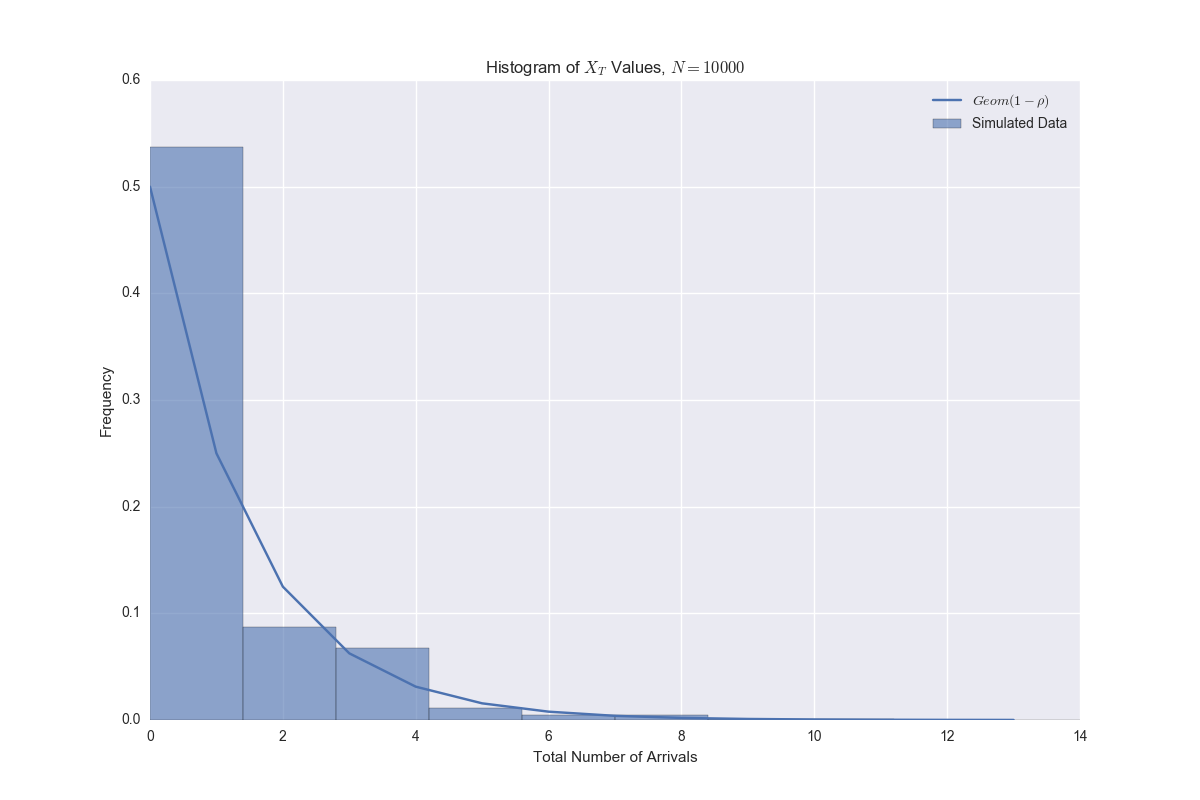
\includegraphics[scale=0.3]{./xt_dist.png}
    \end{figure}

    This looks exactly as we imagined it would.

    \vspace{0.5cm}
    @ Verify your answer in part (3).
    \vspace{0.5cm}

    We can create another histogram.

    \begin{figure}[H]
        \centering
        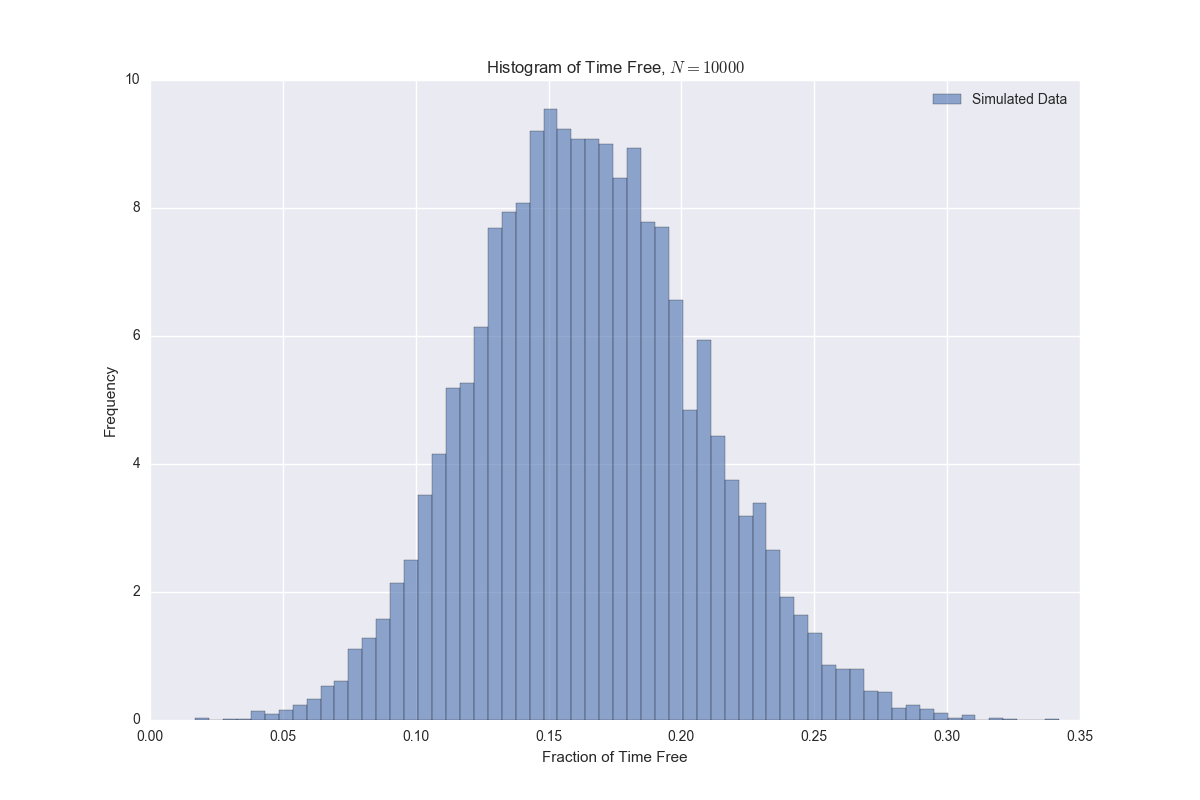
\includegraphics[scale=0.3]{./time_free.png}
    \end{figure}

    I was completely wrong about the distribution here, I had imagined it would
    be simply a ratio of our $\lambda$ to our $\mu$, but these results are
    completely different. Looking up the results online, it turns out that this
    is a modified Bessel function of the first
    kind.\footnote{\url{https://en.wikipedia.org/wiki/M/M/1_queue\#Busy_period_of_server}}

    \vspace{0.5cm}
    @ According to Theorem 4.10, if $X$ is in equilibrium then the output
    process of the queue is a homogeneous Poisson (point) process with intensity
    $\lambda$. Verify by simulating the inter-departure times from the queue.
    \vspace{0.5cm}

    We can draw a similar graph as in the last lab to show the Poisson Point
    Process.

    \begin{figure}[H]
        \centering
        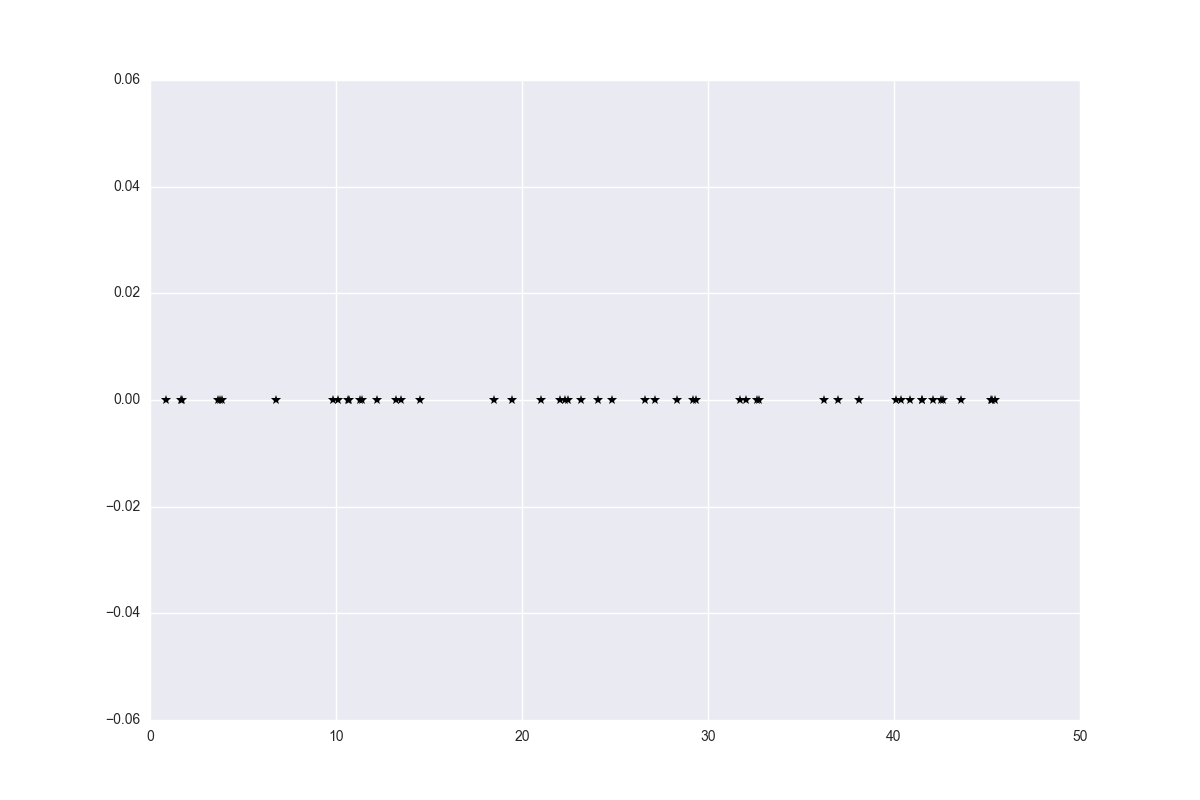
\includegraphics[scale=0.3]{./poissonprocess.png}
    \end{figure}

    This looks exactly like a Poisson Process!

\end{easylist}

\newpage
\appendix
\section{Code}\label{app:code}

\inputminted{python}{lab3.py}
\end{document}
